% =========================================================================
% Stato dei lavori (Web Science 2027): traccia viva di cosa e' stato fatto
% e di cosa faremo. Nata dalla parte "Esperimenti di John" della riunione
% dopo IrForGood (Riunioni/Riunione dopo IrForGood), poi staccata.
% Figure: figure/genera_figure.py (legge Code/WebScience2027).
% Build: tectonic stato_dei_lavori.tex
% =========================================================================
\documentclass[aspectratio=169]{beamer}
\usetheme{Madrid}
\usecolortheme{whale}
\usepackage[T1]{fontenc}
\usepackage{graphicx}
\usepackage{booktabs}
\usepackage{array}
\usepackage{xcolor}
\usepackage{tikz}
\graphicspath{{./figure/}{./}}

\beamertemplatenavigationsymbolsempty
\setbeamercovered{invisible}
\setbeamertemplate{caption}{\insertcaption}
\newcommand{\hl}[1]{\textbf{#1}}
\newenvironment{johnblock}{\begin{exampleblock}{\footnotesize Commento di John}\footnotesize}{\end{exampleblock}}
\newenvironment{claudeblock}{\setbeamercolor{block title}{fg=white,bg=gray!65!black}\setbeamercolor{block body}{bg=gray!12}\begin{block}{\footnotesize Commento di Claude}\footnotesize}{\end{block}}
\newcommand{\divider}[2]{%
  \begin{frame}[plain]
    \vfill
    \begin{center}
      {\color{dividerblue}\Huge\textbf{#1}}\\[0.8em]
      {\large #2}
    \end{center}
    \vfill
  \end{frame}}
\definecolor{wrongred}{RGB}{176,0,32}
\definecolor{dividerblue}{RGB}{28,42,92}
\newcommand{\wrong}[1]{\textcolor{wrongred}{#1}}

\title[Stato dei lavori]{Stato dei lavori}
\subtitle{Web Science 2027: cosa abbiamo fatto e cosa faremo}
\author[John Bianchi]{John Bianchi}
\institute[]{IMT Lucca \& IIT-CNR Pisa}
\date{}

\begin{document}

\begin{frame}
  \titlepage
\end{frame}

\begin{frame}{Il percorso in breve}
  \centering\scriptsize
  \begin{tabular}{>{\raggedright\arraybackslash}p{0.2\textwidth}>{\raggedright\arraybackslash}p{0.33\textwidth}>{\raggedright\arraybackslash}p{0.38\textwidth}}
    \toprule
    \textbf{Fase} & \textbf{La domanda} & \textbf{Il risultato} \\
    \midrule
    Primo dataset (IrForGood, 439 testate) & perch\'e il TF-IDF va come i transformer del paper? & le \hl{reti} di siti gonfiano i numeri: 0,68 $\to$ 0,39 con i fold per gruppo \\
    \addlinespace
    Versione 1 (nuovo dataset, 304 testate) & con pulizia, reti e fold per gruppo, chi vince? & \hl{pari}: TF-IDF F1 0,38, transformer 0,35--0,37 \\
    \addlinespace
    Versione 2 & pi\`u pulizia e pi\`u testate nel training aiutano i transformer? & \hl{no}: niente cambia \\
    \addlinespace
    Analisi del TF-IDF & come fa ad andare cos\`i bene? & legge il \hl{genere} della testata (orientamento, tipo di sito, paese) \\
    \addlinespace
    Versione 3 & a parit\`a di genere, il testo dice l'affidabilit\`a? & s\`i, ma poco (0,6 contro 0,5), ed \`e \hl{stile}; il TF-IDF resta davanti \\
    \addlinespace
    Versione 4 & il titolo letto con l'articolo e i criteri NewsGuard aiutano i transformer? & un po', ma il titolo aiuta \hl{anche} il TF-IDF: il distacco resta \\
    \addlinespace
    Oltre il testo & i link citati e la pagina HTML aiutano? & \hl{no}: tutto arriva a F1 circa 0,34, binario circa 0,70 \\
    \bottomrule
  \end{tabular}\\[0.6em]
  \raggedright{\small\itshape Sotto, ogni fase con i dettagli.}
\end{frame}

% ===================================================================================================
\divider{Il primo dataset}{dai transformer del paper a un classificatore pi\`u semplice}

\begin{frame}{Il punto di partenza: i transformer del paper}
  \vfill
  \begin{itemize}[<+->]
    \setlength\itemsep{0.8em}
    \item Il dataset di IrForGood: \hl{439 testate}, \hl{19.476 articoli}; 5 fold, nel test solo testate \hl{mai viste} in addestramento
    \item \hl{Per articolo}: accuratezza intorno a \hl{0,60} (da 0,58 di BERT a 0,61 di Mistral), F1 macro 0,52--0,55
    \item \hl{Per testata} (voto di maggioranza dei suoi articoli): accuratezza fino a \hl{0,69} (RoBERTa; Mistral 0,68), tolerant 1 fino a 0,88
    \item[] {\small\itshape Modelli da 110 milioni a 24 miliardi di parametri, tutti pi\`u o meno allo stesso livello.}
  \end{itemize}
  \vfill
\end{frame}

\begin{frame}{Un classificatore a feature fa lo stesso, se non meglio}
  \begin{itemize}[<+->]
    \setlength\itemsep{0.5em}
    \item \hl{TF-IDF}: ogni articolo diventa l'elenco delle sue parole (e coppie di parole), pesate per quanto sono rare; sopra, una \hl{regressione logistica}. Nessuna rete neurale: si addestra in un minuto
    \item Sugli \hl{stessi fold} del paper:
  \end{itemize}
  \vspace{0.3em}
  \visible<3->{%
  \centering\small
  \begin{tabular}{lcccc}
    \toprule
    & \multicolumn{2}{c}{\textbf{per articolo}} & \multicolumn{2}{c}{\textbf{per testata}} \\
    \cmidrule(lr){2-3}\cmidrule(lr){4-5}
    & accuratezza & F1 macro & accuratezza & tolerant 1 \\
    \midrule
    migliore dei 4 transformer (misura per misura) & 0,61 & 0,55 & 0,69 & 0,88 \\
    \textbf{TF-IDF + regressione logistica} & 0,58 & 0,52 & \textbf{0,68} & \textbf{0,88} \\
    \bottomrule
  \end{tabular}\par}
  \vspace{0.6em}
  \begin{itemize}[<+->]
    \setcounter{beamerpauses}{4}
    \item Come fa un modello che \hl{conta parole} ad andare come Mistral da 24 miliardi di parametri?
    \item Per capirlo ho guardato \hl{dentro il dataset}
  \end{itemize}
\end{frame}

\begin{frame}{Quanto si somigliano due articoli? (1) I pezzetti di 5 parole}
  \begin{itemize}[<+->]
    \setlength\itemsep{0.6em}
    \item Il testo si \hl{normalizza}: minuscole, niente punteggiatura, i numeri diventano \#
    \item Poi si spezza in tutti i \hl{pezzetti di 5 parole consecutive}:
    \item[] {\small\ttfamily there was a single gas station in cities across phillips county}\\[0.2em]
            {\small $\to$ \ttfamily [there was a single gas] [was a single gas station] [a single gas station in] \dots}
    \item \hl{Somiglianza di Jaccard} tra due articoli $A$ e $B$:
    \[ J(A,B) = \frac{\text{pezzetti in comune}}{\text{pezzetti di tutti e due, contati una volta}} = \frac{|A \cap B|}{|A \cup B|} \]
    \item $J = 0$: niente in comune; $J = 1$: lo stesso testo. \hl{$J \geq 0{,}5$}: pi\`u di met\`a dei pezzetti in comune, gli articoli sono \hl{quasi uguali} (non per forza identici)
  \end{itemize}
\end{frame}

\begin{frame}{Quanto si somigliano due articoli? (2) Un esempio vero}
  \begin{columns}[t]
    \begin{column}{0.48\textwidth}
      \begin{block}{\footnotesize ncindiananews.com}
        \scriptsize Federal Energy Regulatory Commission (FERC) Commissioner Mark C. Christie \textbar{} www.ferc.gov\\[0.3em]
        There was a single gas station in cities across \hl{White County} selling premium gas at the lowest price of \hl{\$3.81} per gallon \dots
      \end{block}
    \end{column}
    \begin{column}{0.48\textwidth}
      \begin{block}{\footnotesize savannahstandard.com}
        \scriptsize Federal Energy Regulatory Commission (FERC) Commissioner Mark C. Christie \textbar{} www.ferc.gov\\[0.3em]
        There were two gas stations in cities across \hl{Bulloch County} selling premium gas at the lowest price of \hl{\$3.79} per gallon \dots
      \end{block}
    \end{column}
  \end{columns}
  \vspace{0.6em}
  \begin{itemize}[<+->]
    \setlength\itemsep{0.5em}
    \item Due siti diversi, lo \hl{stesso articolo-modello}: cambiano solo la contea e i numeri
    \item Sono articoli \hl{generati in serie} da una rete di siti locali: il testo \`e quasi tutto uguale ($J$ tra 0,6 e 1)
    \item Un classificatore che ha visto uno di questi nel training riconosce subito l'altro nel test
  \end{itemize}
\end{frame}

\begin{frame}{Quanto si somigliano due articoli? (3) Confrontarli tutti}
  \vfill
  \begin{itemize}[<+->]
    \setlength\itemsep{0.8em}
    \item 19.476 articoli sono quasi \hl{190 milioni di coppie}: calcolare $J$ esatto su tutte, testo contro testo, \`e \hl{impossibile} in tempi ragionevoli
    \item \hl{MinHash} e \hl{LSH} servono a questo: calcolano la somiglianza di Jaccard in modo \hl{fattibile}, accettando una piccola \hl{approssimazione}
    \item[] MinHash riassume ogni articolo in un'\hl{impronta} corta da cui si stima $J$; LSH propone solo le coppie che \hl{probabilmente} si somigliano
    \item[] {\small\itshape \`E la tecnica standard per togliere i duplicati dai dati di addestramento dei modelli linguistici.}
    \item Risultato: \hl{1.557} articoli hanno una copia \hl{identica} su un'altra testata; \hl{4.740} (il \hl{24\%}) una copia \hl{quasi uguale} ($J \geq 0{,}5$)
  \end{itemize}
  \vfill
\end{frame}

\begin{frame}{Dagli articoli alle reti di testate}
  \begin{columns}[c]
    \begin{column}{0.42\textwidth}
      \begin{itemize}[<+->]
        \setlength\itemsep{0.6em}
        \item Due testate sono \hl{collegate} se hanno \hl{almeno 2 articoli} quasi uguali in comune (una sola copia pu\`o essere un pezzo ripreso)
        \item Una \hl{rete} = testate collegate anche \hl{a catena}: A--B e B--C $\Rightarrow$ A, B, C nella stessa rete
        \item \hl{10 reti}, con dentro \hl{236 testate su 439}; la pi\`u grande ha \hl{131 siti}
      \end{itemize}
    \end{column}
    \begin{column}{0.58\textwidth}
      \centering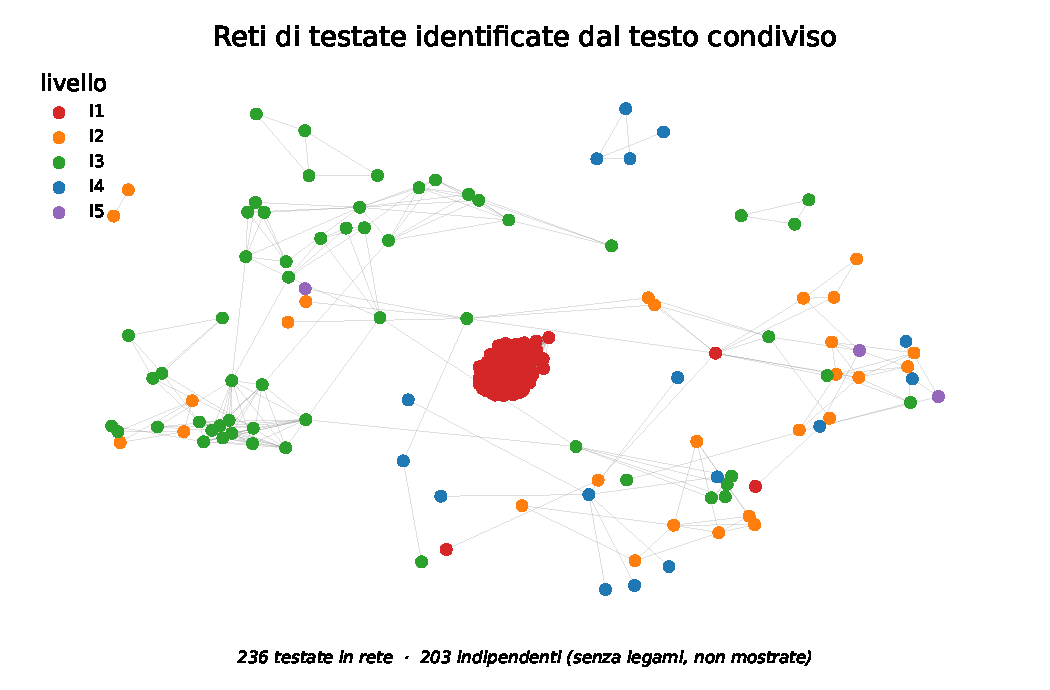
\includegraphics[width=\textwidth]{fig_primo_rete.pdf}\\
      {\scriptsize Un punto = una testata; una linea = almeno 2 articoli quasi uguali. La distanza nel disegno non misura nulla.}
    \end{column}
  \end{columns}
\end{frame}

\begin{frame}{Chi c'\`e dietro una rete: l'owner di NewsGuard}
  \vfill
  \begin{itemize}[<+->]
    \setlength\itemsep{0.7em}
    \item Per ogni sito NewsGuard indica anche il \hl{proprietario} (campo \hl{Owner}): per esempio Metric Media LLC, Boone Newspapers, Salem Media Group
    \item Le reti le ho trovate \hl{solo dal testo}; l'owner l'ho usato \hl{dopo}, per controllarle:
    \item[] \hl{precisione 0,93}: le testate di una stessa rete hanno quasi sempre lo stesso proprietario
    \item[] \hl{recall 0,87}: le testate di uno stesso proprietario finiscono quasi sempre nella stessa rete
    \item La rete da 131 siti: \hl{tutti di Metric Media LLC}, tutti con lo \hl{stesso punteggio} NewsGuard (32): siti di ``notizie locali'' che pubblicano articoli-modello come quello di prima
    \item[] {\small\itshape Quindi: stessa rete = testo quasi uguale (non sempre identico) e, quasi sempre, stesso proprietario.}
  \end{itemize}
  \vfill
\end{frame}

\begin{frame}{Le reti, livello per livello}
  \centering
  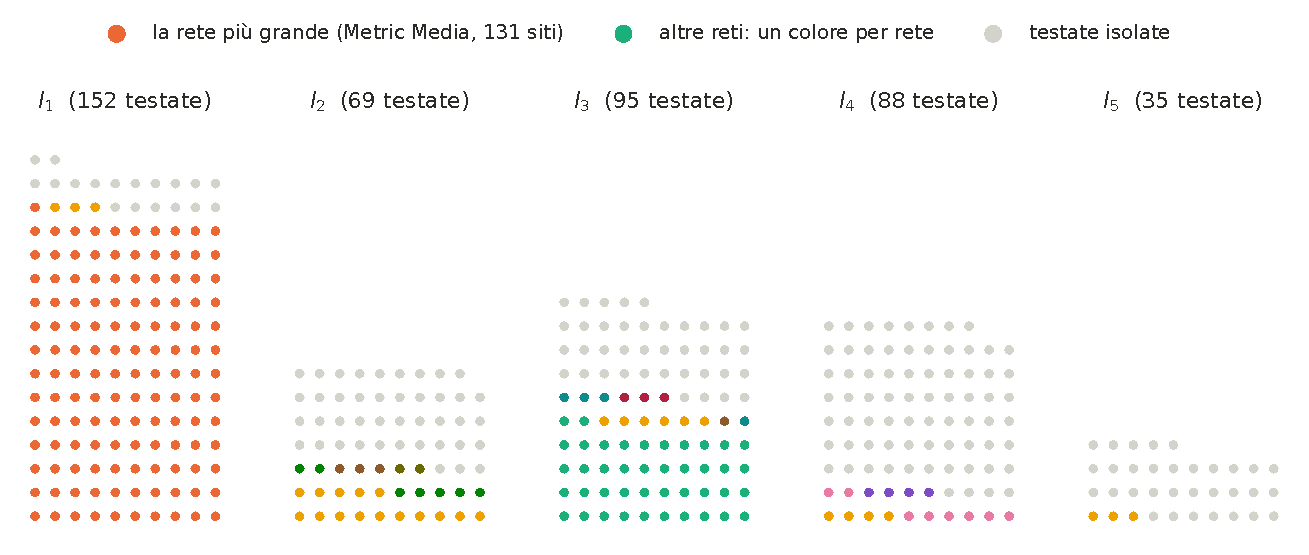
\includegraphics[height=0.56\textheight]{fig_primo_puntini_livelli.pdf}\\[0.1em]
  {\footnotesize Un pallino = una testata; un colore = una rete.}
  \begin{itemize}[<+->]
    \small
    \item $l_1$: \hl{131 testate su 152} sono la stessa rete di Metric Media; solo \hl{20} sono isolate
    \item $l_3$: molte catene di giornali locali; $l_4$ e $l_5$: quasi tutte isolate
  \end{itemize}
\end{frame}

\begin{frame}{Fold per testata: le sorelle stanno da tutte e due le parti}
  \centering
  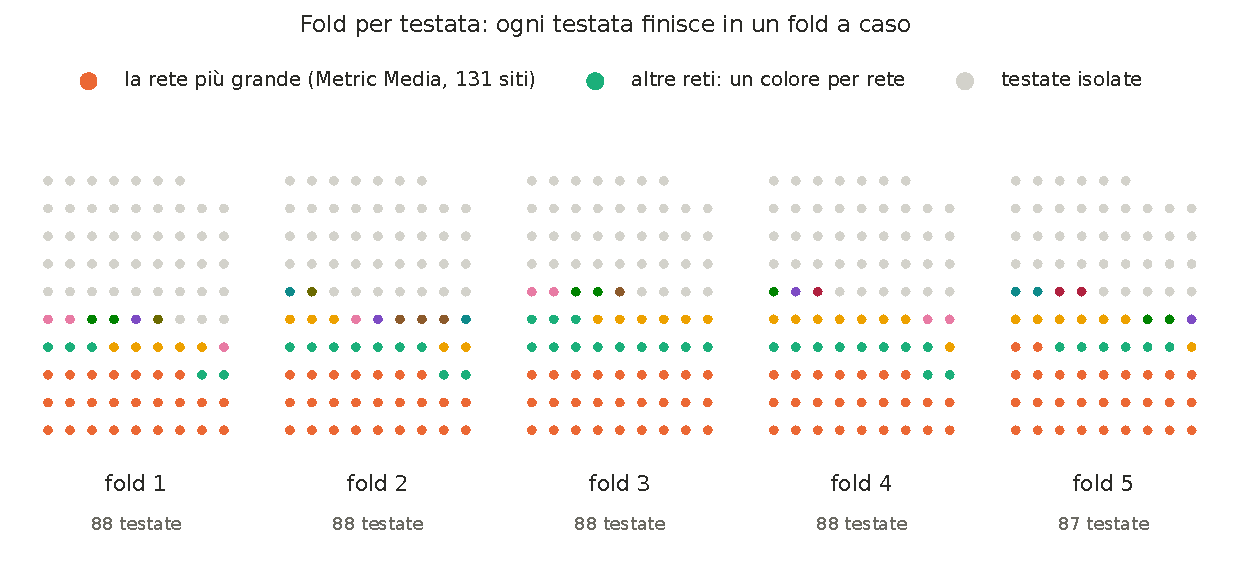
\includegraphics[height=0.56\textheight]{fig_primo_fold_testata.pdf}\\[0.1em]
  \begin{itemize}[<+->]
    \small
    \item Come nel paper: ogni testata va in un fold \hl{a caso}, e i 131 siti di Metric Media si spargono in \hl{tutti e 5} i fold (25--29 per fold)
    \item Lo stesso per le altre reti: ogni colore compare in pi\`u fold, in media \hl{3,5}
    \item Quando il fold 1 \`e il test, gli altri \hl{106 siti} di Metric Media sono nel training: il modello ha gi\`a visto gli stessi articoli-modello
  \end{itemize}
\end{frame}

\begin{frame}{Ripulire il primo dataset: cosa ho tolto e come}
  \vspace{0.2em}
  \centering\footnotesize
  \begin{tabular}{p{0.04\textwidth}p{0.34\textwidth}p{0.25\textwidth}p{0.25\textwidth}}
    \toprule
    & \textbf{Regola} & \textbf{Con quale indice} & \textbf{Quanto} \\
    \midrule
    1 & lo stesso articolo su pi\`u testate: se ne tiene \hl{una copia} & $J \geq 0{,}9$ (stesso testo con poche parole cambiate) & $-$1.835 articoli \\
    2 & copie rimaste tra \hl{reti diverse}: si tolgono tutte e due & $J \geq 0{,}5$ & $-$46 articoli \\
    3 & \hl{paragrafi identici} in almeno 2 testate (didascalie, appelli, avvisi): tolti \hl{dal testo}, l'articolo resta & uguaglianza del paragrafo normalizzato & 5,5\% delle parole \\
    4 & articoli rimasti con \hl{100 parole o meno} & --- & $-$1.325 articoli \\
    \bottomrule
  \end{tabular}\\[0.5em]
  \raggedright
  \begin{itemize}[<+->]
    \item Verifica: coppie di articoli quasi uguali tra reti diverse, rifacendo il MinHash sul testo pulito: da \hl{1,45 milioni} a \hl{0}
    \item Le regole \hl{non guardano le etichette}: si applicano uguali a tutti i livelli
  \end{itemize}
\end{frame}

\begin{frame}{Pulito e valutato per gruppo, il primo dataset non basta}
  \begin{columns}[c]
    \begin{column}{0.56\textwidth}
      \centering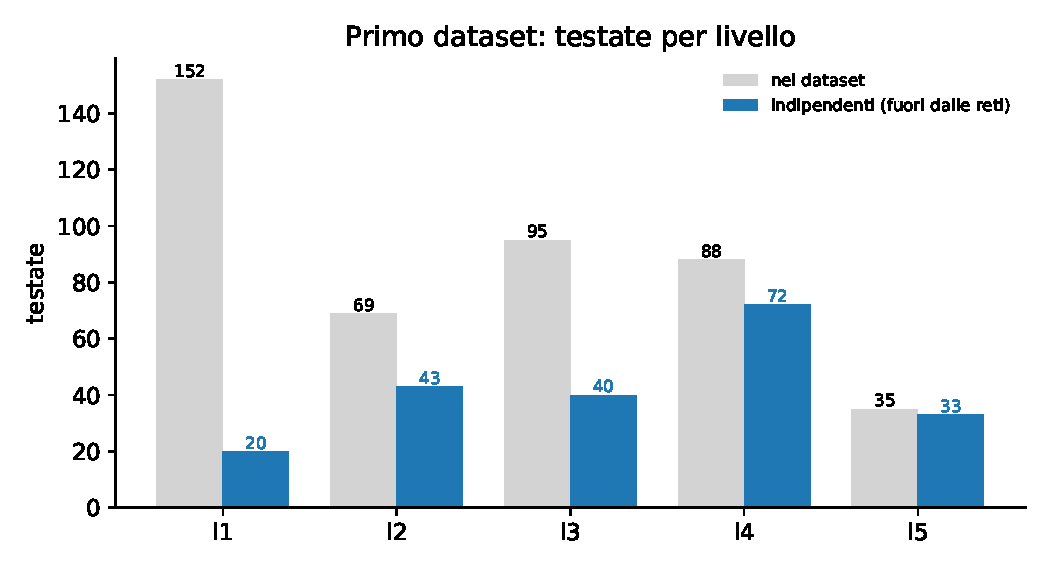
\includegraphics[width=\textwidth]{fig_primo_prima_dopo.pdf}
    \end{column}
    \begin{column}{0.44\textwidth}
      \begin{itemize}[<+->]
        \setlength\itemsep{0.6em}
        \item TF-IDF sul dataset pulito, fold per gruppo: \hl{0,40} di accuratezza, \hl{0,33} di F1 macro
        \item Testate \hl{indipendenti} (fuori dalle reti): solo \hl{20 $l_1$}; il resto di $l_1$ \`e una rete sola, che conta come \hl{un} esempio
        \item Troppo poche testate indipendenti per livello: per andare avanti serve un \hl{dataset nuovo}, pi\`u grande, pulito con lo stesso rigore
      \end{itemize}
    \end{column}
  \end{columns}
\end{frame}

% ===================================================================================================
\divider{Il nuovo dataset}{come l'ho costruito, passo per passo}

\begin{frame}{Lo scraping: due giri nella stessa settimana}
  \begin{itemize}[<+->]
    \setlength\itemsep{0.6em}
    \item \hl{13 ottobre}, primo giro: le testate NewsGuard in inglese, con un punteggio, il cui argomento \`e \hl{esattamente} ``Political news or commentary'': \hl{1.921}
    \item Non bastano: molti siti \hl{bloccano} lo scraper, molti articoli \hl{sporchi} si tolgono, e il tetto di \hl{5 testate per gruppo} (rete o stesso owner, passo 3) ne scarta tante. Serve il dataset \hl{pi\`u grande possibile}
    \item \hl{18 ottobre}, secondo giro, \hl{stesso scraper} e stessi parametri: le testate il cui argomento \hl{contiene} ``Political news or commentary'' insieme ad altri: \hl{+1.207}. Nessuna testata in comune: gli articoli dei due giri si \hl{sommano}
    \item In tutto \hl{3.128} testate tentate, \hl{1.528} raggiunte (bloccata quasi tutta una rete di 1.076 siti $l_1$, pi\`u 176 altre)
    \item In \hl{ordine casuale} e \hl{senza guardare il livello}; fino a 200 articoli recenti per testata, con l'\hl{HTML grezzo}
    \item I due giri sono a \hl{5 giorni} di distanza, con lo stesso strumento: un dataset \hl{coerente}
  \end{itemize}
\end{frame}

\begin{frame}{Prima di questo dataset: altri tentativi}
  \vfill
  \begin{itemize}[<+->]
    \setlength\itemsep{0.9em}
    \item Prima di arrivare qui ho fatto \hl{altri tentativi}, provando \hl{pi\`u strategie di pulizia}
    \item Ogni volta il feature \hl{batteva ancora} i transformer, e in parte per lo \hl{sporco} rimasto nel dataset: testo del sito ripetuto in tutti gli articoli, pagine uguali per tutta una testata, reti di siti non separate
    \item Allora ho reso la pulizia \hl{pi\`u aggressiva}: non pi\`u solo le copie tra testate, come nel primo dataset, ma anche il testo che appartiene al sito e non all'articolo, e le reti trovate anche dall'HTML
    \item Con un limite: si toglie solo quello che \hl{non \`e dell'articolo}; citazioni e pezzi ripresi restano
  \end{itemize}
  \vfill
\end{frame}

\begin{frame}{Come ho costruito il dataset, in breve}
  \vfill
  \begin{enumerate}[<+->]
    \setlength\itemsep{1em}
    \item \hl{Pulire il testo degli articoli}: togliere quello che non \`e dell'articolo ma \hl{del sito} (appelli, firme, titolo ripetuto, data). Un modello lo userebbe per riconoscere il sito, non l'affidabilit\`a
    \item \hl{Trovare le testate parenti} (le reti), \hl{senza guardare NewsGuard}: dalle tracce che lasciano, come testi uguali, stessi codici nell'HTML, stessi autori
    \item \hl{Fare i gruppi e i fold}: le testate parenti vanno tutte dalla stessa parte, e nessun gruppo pu\`o essere troppo grande
  \end{enumerate}
  \vfill
  \visible<4->{\small Ogni passo \`e una \hl{regola scritta nel codice}, applicata uguale a tutte le testate: \hl{nessun testo tolto a mano} o da un LLM. Rieseguendo i notebook (random state fissati) dai dati dello scraping esce sempre lo stesso dataset.}
\end{frame}

\begin{frame}{1. Pulire gli articoli}
  \begin{itemize}[<+->]
    \setlength\itemsep{0.5em}
    \small
    \item Si toglie dal testo quello che \hl{appartiene al sito}, non all'articolo:
    \item[] le frasi che si \hl{ripetono} in molti articoli della stessa testata: appelli, firme, ``iscriviti alla newsletter''. Per esempio truthout.org ha lo stesso appello per le donazioni in \hl{200 articoli su 200}
    \item[] la \hl{cornice della pagina}: il titolo e la data che alcuni siti mettono all'inizio del testo
    \item Si tolgono gli articoli \hl{vecchi} (prima del 2025), i \hl{doppioni} dello stesso pezzo e quelli rimasti \hl{troppo corti}
    \item Sono \hl{impronte del sito}: lasciate l\`i, un modello riconoscerebbe la testata invece di leggere l'articolo
    \item Tutto con \hl{regole automatiche} nel codice, nessuna modifica a mano. Risultato: via il 5\% delle parole; da 101.887 a \hl{76.091} articoli
    \item[] {\small\itshape Con lo stesso MinHash del primo dataset si trovano anche le copie tra testate: servono al passo 2.}
  \end{itemize}
\end{frame}

\begin{frame}{2. Trovare le testate parenti: le tracce}
  \vspace{0.1em}
  \centering\scriptsize
  \begin{tabular}{p{0.15\textwidth}p{0.52\textwidth}p{0.24\textwidth}}
    \toprule
    \textbf{Traccia} & \textbf{Quando due testate sono parenti} & \textbf{Esempio} \\
    \midrule
    copie & hanno articoli quasi uguali in comune (MinHash, $J \geq 0{,}5$): almeno 2, e almeno il 10\% degli articoli della pi\`u piccola & catene di giornali locali \\
    codici\newline di account & nell'HTML di ogni pagina c'\`e il \hl{numero di conto} di AdSense, Google Analytics, pixel di Facebook\dots{} (es.\ \texttt{ca-pub-1234\dots}): due siti con \hl{lo stesso numero} usano lo stesso conto. Conta solo se \`e in almeno met\`a delle pagine & FiveZero: 18 siti, un solo conto AdSense \\
    privacy policy & il link ``Privacy policy'' porta alla \hl{stessa pagina} su un altro dominio, cio\`e lo stesso titolare. Non contano Google, WordPress, Substack e simili, uguali per tutti i clienti & 8 siti, tutti verso la privacy policy di \texttt{salemmedia.com} \\
    dominio & sottodomini dello stesso sito, o la homepage che \hl{reindirizza} allo stesso dominio & le edizioni di HuffPost \\
    autori & la firma dell'articolo: gli \hl{stessi nomi di persona} (non ``Staff'' o le agenzie) firmano almeno il 10\% degli articoli della pi\`u piccola & la rete da 426 siti \\
    \bottomrule
  \end{tabular}\\[0.5em]
  \raggedright\footnotesize
  \begin{itemize}[<+->]
    \item Basta \hl{una} traccia per collegare due testate; una \hl{rete} = testate collegate, anche a catena (come nel primo dataset)
    \item Le soglie del 10\% evitano di collegare due testate per un pezzo d'agenzia o un collaboratore in comune
  \end{itemize}
\end{frame}

\begin{frame}{2. Le reti trovate}
  \begin{columns}[c]
    \begin{column}{0.62\textwidth}
      \centering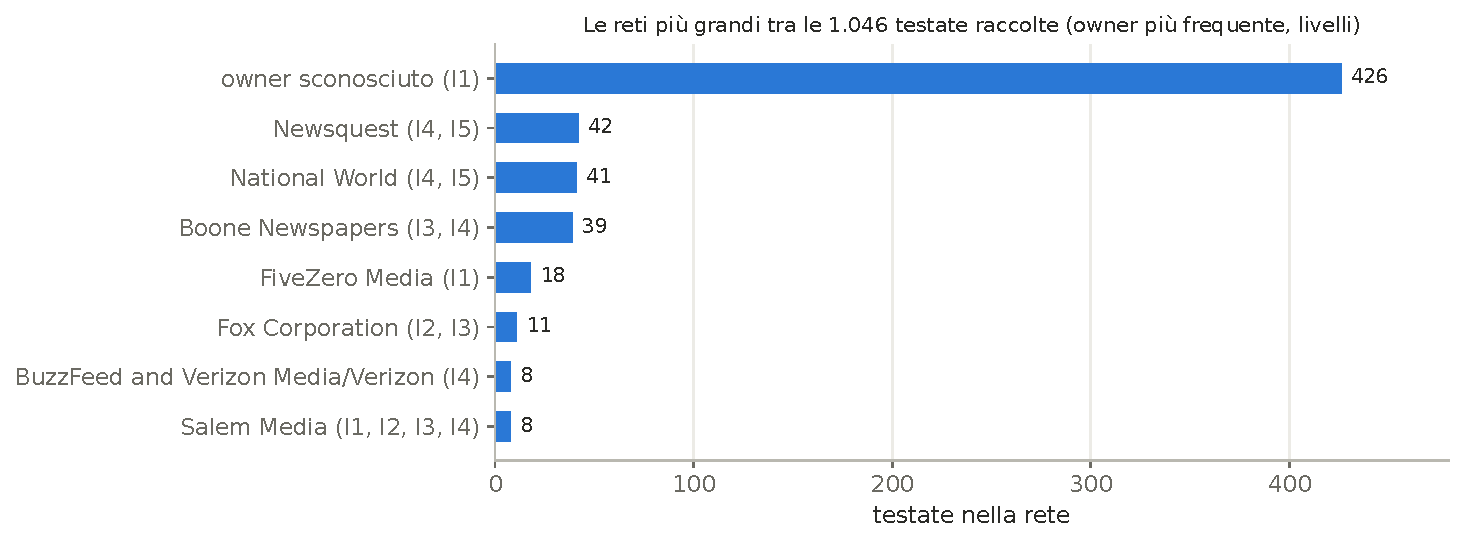
\includegraphics[width=\textwidth]{fig_reti_grandi.pdf}
    \end{column}
    \begin{column}{0.38\textwidth}
      \begin{itemize}[<+->]
        \setlength\itemsep{0.6em}
        \small
        \item \hl{725 testate su 1.046} stanno in una rete con altre
        \item La pi\`u grande ha \hl{426 siti}, legati soprattutto dagli \hl{stessi autori}. Per NewsGuard l'owner \`e \hl{sconosciuto}
        \item Controllo a parte: tutti hanno lo \hl{stesso punteggio} (5) e nel campo ``Parent Domain'' di NewsGuard \hl{425 su 426} dicono \texttt{naturalnews.com}. \`E la rete di Natural News
      \end{itemize}
    \end{column}
  \end{columns}
\end{frame}

\begin{frame}{2. Il controllo con l'owner di NewsGuard}
  \begin{columns}[c]
    \begin{column}{0.54\textwidth}
      \centering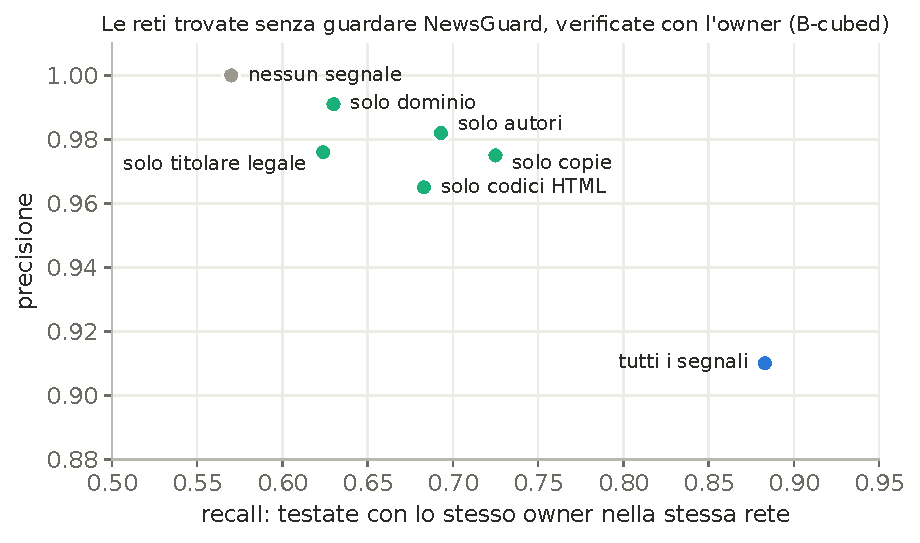
\includegraphics[width=\textwidth]{fig_reti_verifica.pdf}
    \end{column}
    \begin{column}{0.46\textwidth}
      \begin{itemize}[<+->]
        \setlength\itemsep{0.5em}
        \small
        \item Le reti le ho trovate \hl{senza} l'owner: ora lo uso per vedere se sono giuste
        \item Per ogni testata con un owner noto:
        \item[] \hl{precisione}: le testate della sua rete hanno il suo stesso owner?
        \item[] \hl{recall}: le testate del suo owner sono nella sua rete?
        \item[] e poi la media su tutte le testate
        \item Ogni traccia da sola \`e precisa ma trova poco; \hl{tutte insieme}: precisione \hl{0,91}, recall \hl{0,88}
        \item Le testate con owner sconosciuto non entrano nel conto: si controllano a parte, come Natural News
      \end{itemize}
    \end{column}
  \end{columns}
\end{frame}

\begin{frame}{3. I gruppi}
  \vfill
  \begin{itemize}[<+->]
    \setlength\itemsep{1em}
    \item \hl{Gruppo} = rete trovata \hl{oppure} stesso owner NewsGuard: basta uno dei due. L'owner aggiunge le parentele che non lasciano tracce
    \item Lo stesso articolo in \hl{due gruppi diversi}: si tiene la copia pi\`u vecchia ($-$461 articoli). Cos\`i lo stesso testo non sta mai nel training e nel test
    \item Testate con almeno \hl{20 articoli} (per il voto di maggioranza): \hl{702}
  \end{itemize}
  \vfill
\end{frame}

\begin{frame}{3. I gruppi, livello per livello}
  \centering
  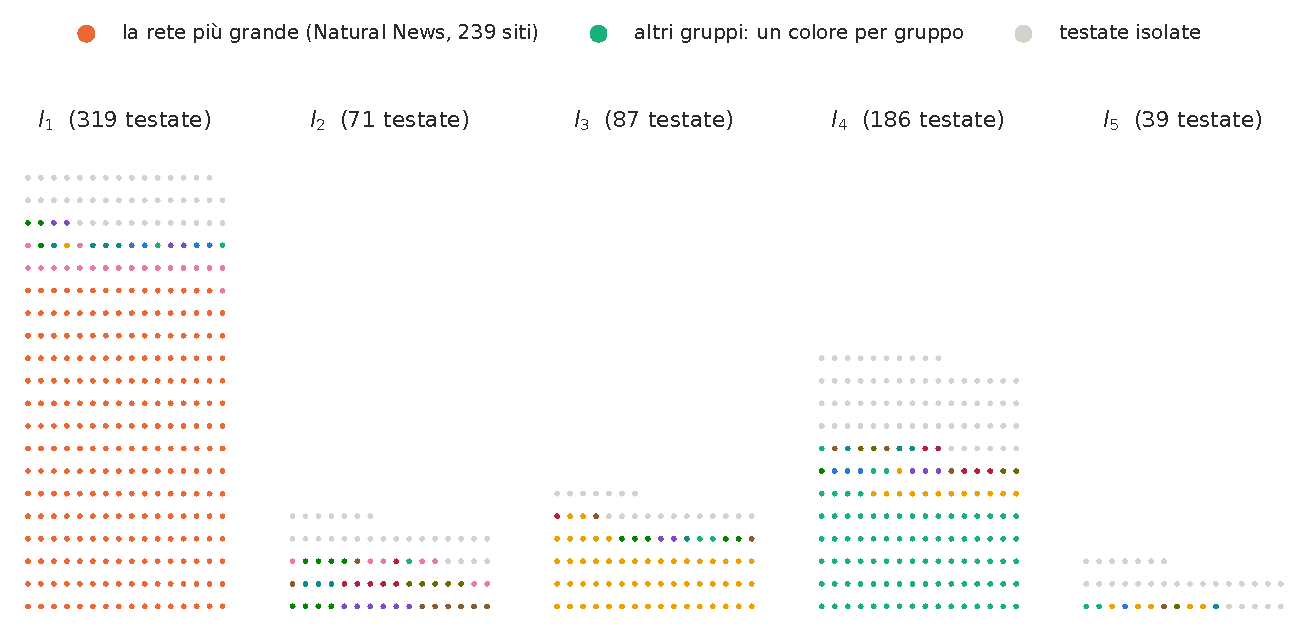
\includegraphics[height=0.6\textheight]{fig_nuovo_prima_tetto.pdf}\\[0.2em]
  {\footnotesize Le 702 testate con almeno 20 articoli. Un pallino = una testata; un colore = un gruppo.}
  \begin{itemize}[<+->]
    \small
    \item Natural News fa \hl{239 delle 319} testate $l_1$: lo stesso problema di Metric Media nel primo dataset
  \end{itemize}
\end{frame}

\begin{frame}{3. Il tetto e i fold}
  \begin{columns}[c]
    \begin{column}{0.5\textwidth}
      \begin{itemize}[<+->]
        \setlength\itemsep{0.7em}
        \item Al massimo \hl{5 testate per gruppo}, scelte \hl{a caso}: Natural News conta come gli altri gruppi, non riempie pi\`u $l_1$
        \item Restano \hl{304 testate} in \hl{220 gruppi}
        \item \hl{5 fold per gruppo}: ogni gruppo sta in un fold solo, e ogni fold ha lo stesso numero di testate per livello
      \end{itemize}
    \end{column}
    \begin{column}{0.5\textwidth}
      \centering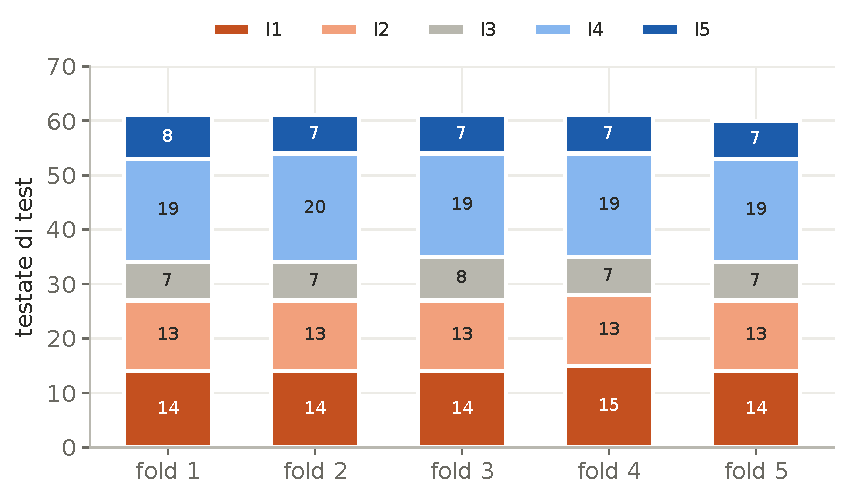
\includegraphics[width=\textwidth]{fig_fold_bilanciati.pdf}\\
      {\footnotesize Testate per livello in ogni fold di test}
    \end{column}
  \end{columns}
\end{frame}

\begin{frame}{Quanto resta a ogni passo}
  \centering
  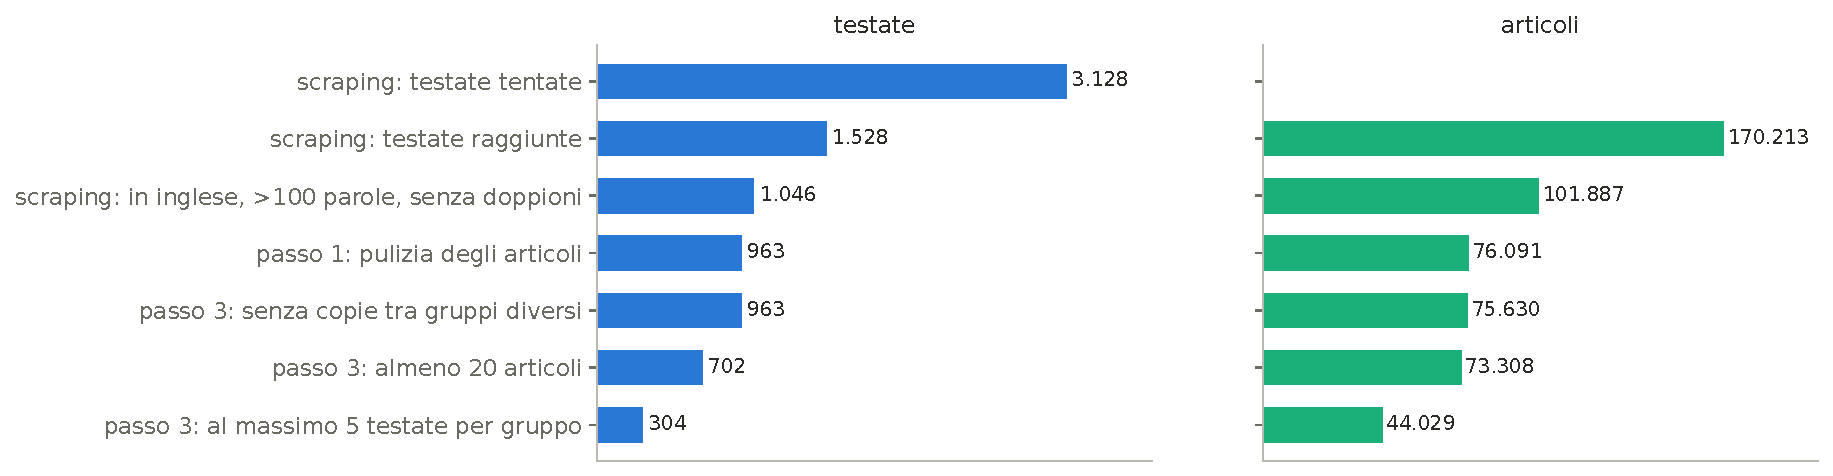
\includegraphics[width=0.96\textwidth]{fig_nuovo_imbuto.pdf}\\[0.4em]
  {\footnotesize Il passo 2 non toglie articoli: serve a fare i gruppi.}
\end{frame}

\begin{frame}{Il dataset finale}
  \centering
  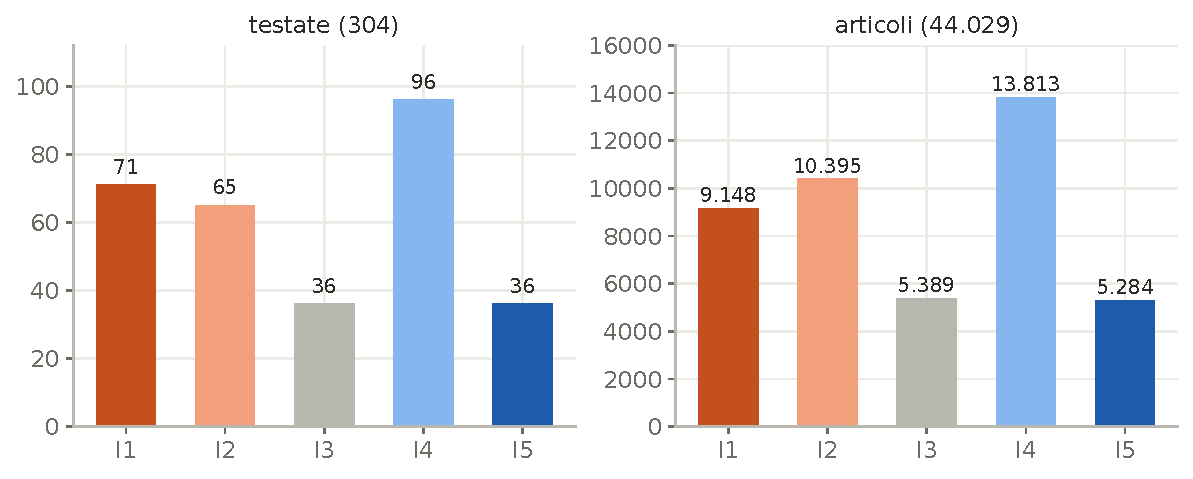
\includegraphics[width=0.85\textwidth]{fig_nuovo_composizione.pdf}\\[0.4em]
  \begin{itemize}[<+->]
    \item \hl{304 testate}, \hl{44.029 articoli}, \hl{220 gruppi} indipendenti
    \item Pi\`u del doppio delle testate $l_1$ indipendenti rispetto al primo dataset (56 gruppi contro 20)
  \end{itemize}
\end{frame}

% ===================================================================================================
\divider{La sporcizia \`e andata?}{gli stessi grafici, sul dataset nuovo}

\begin{frame}{Le reti livello per livello, ora}
  \centering
  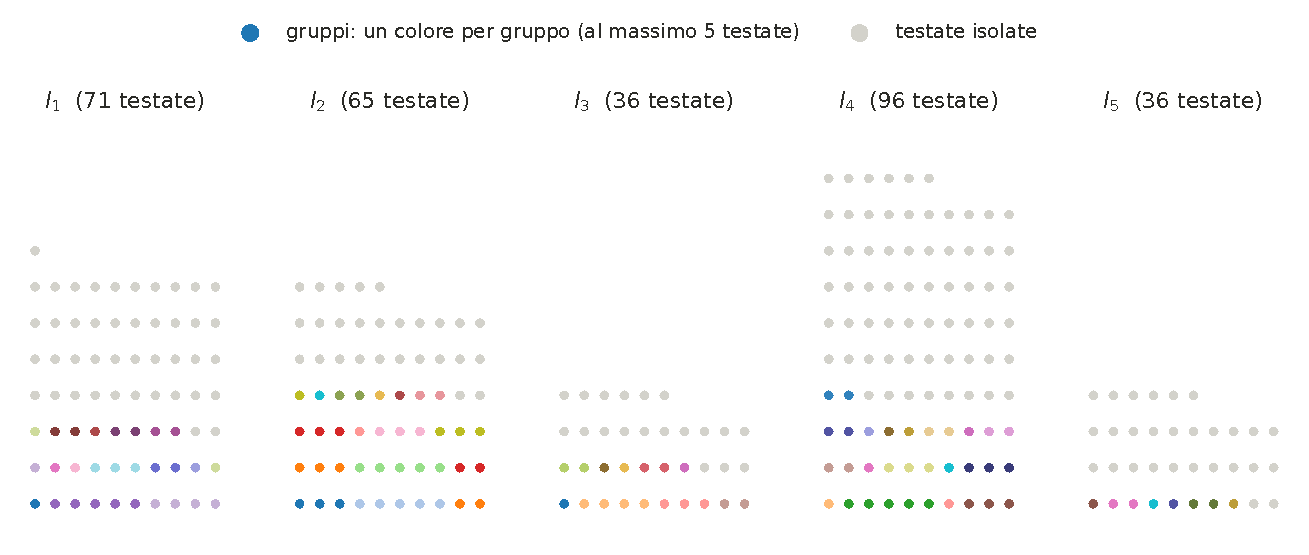
\includegraphics[height=0.56\textheight]{fig_nuovo_puntini_livelli.pdf}\\[0.1em]
  {\footnotesize Un pallino = una testata; un colore = un gruppo.}
  \begin{itemize}[<+->]
    \small
    \item Prima: \hl{131 testate $l_1$ su 152} erano una rete sola. Ora nessun gruppo ha pi\`u di \hl{5 testate}
    \item \hl{181 testate isolate} e \hl{123} in 39 gruppi piccoli; in $l_1$, 43 isolate su 71
  \end{itemize}
\end{frame}

\begin{frame}{I fold, ora}
  \centering
  \only<1>{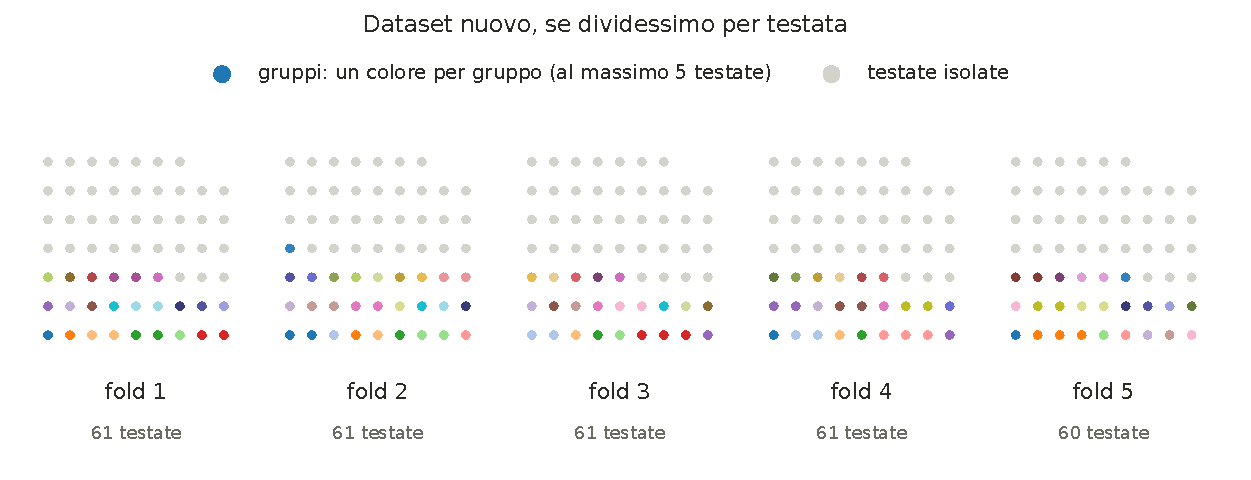
\includegraphics[height=0.5\textheight]{fig_nuovo_fold_testata.pdf}}%
  \only<2->{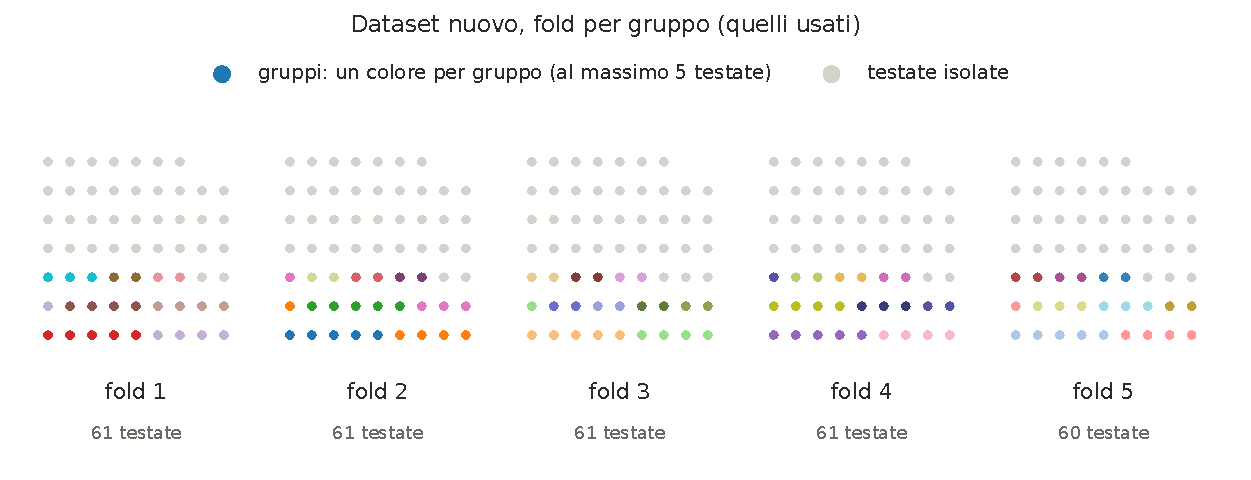
\includegraphics[height=0.5\textheight]{fig_nuovo_fold_gruppo.pdf}}\\[0.1em]
  \begin{itemize}
    \small
    \item<1-> Se dividessimo \hl{per testata}, un gruppo starebbe in media in \hl{2,4 fold}: le sorelle di nuovo da tutte e due le parti
    \item<2-> Con i fold \hl{per gruppo} (quelli usati) ogni colore sta in \hl{un solo fold}
    \item<3-> \`E una divisione \hl{in pi\`u}, non al posto di quella per testata: gli articoli di una testata stanno \hl{sempre} in un solo fold, e in pi\`u le testate di un gruppo stanno insieme
  \end{itemize}
\end{frame}

% ===================================================================================================
\divider{Versione 1: i risultati}{TF-IDF contro transformer, sul dataset nuovo (18 ottobre)}

\begin{frame}{I modelli a confronto, in breve}
  \begin{itemize}[<+->]
    \setlength\itemsep{0.6em}
    \small
    \item \hl{TF-IDF + regressione logistica}: parole e coppie di parole pesate per rarit\`a; il parametro di regolarizzazione scelto in una validazione sul solo training (\hl{riferimento}, fissato prima)
    \item \hl{ModernBERT} (base 150M e large 400M parametri), \hl{fine-tuning}: impara a dire il livello di ogni articolo; la testata \`e la media delle probabilit\`a dei suoi articoli
    \item[] La ricetta, uguale per tutti e nata dai tentativi precedenti: primi 1024 token, 2 epoche fisse (l'early stopping su poche testate sceglieva quasi a caso), 20 articoli a caso per testata a ogni epoca, pesi di classe
    \item[] Ogni ModernBERT con \hl{3 seed}: tra un seed e l'altro la F1 cambia di 3--5 punti, quindi il risultato principale \`e l'\hl{ensemble} (media delle probabilit\`a dei 3 modelli)
    \item \hl{Embedding congelati} (e5-large, bge-large): nessun addestramento, un vettore per articolo, media per testata e la stessa regressione logistica del TF-IDF
  \end{itemize}
\end{frame}

\begin{frame}{I risultati della Versione 1}
  \vspace{0.2em}
  \centering\footnotesize
  \begin{tabular}{lcccc}
    \toprule
    \textbf{Modello} & \textbf{F1 macro} & \textbf{accuratezza} & \textbf{tolerant 1} & \textbf{binario} \\
    \midrule
    \textbf{TF-IDF} (riferimento) & \textbf{0,380} & 0,424 & 0,770 & 0,740 \\
    TF-IDF, parametri di default & 0,368 & \textbf{0,454} & \textbf{0,803} & \textbf{0,776} \\
    \midrule
    ModernBERT-base, ensemble di 3 seed & 0,366 & 0,398 & 0,780 & 0,717 \\
    ModernBERT-large, ensemble di 3 seed & 0,348 & 0,405 & 0,799 & 0,743 \\
    \midrule
    e5-large / bge-large congelati & 0,331 / 0,325 & 0,391 / 0,382 & 0,786 / 0,789 & 0,727 / 0,730 \\
    \midrule
    classe di maggioranza / a caso & 0,096 / 0,214 & 0,316 / 0,243 & 0,553 / 0,533 & 0,553 / 0,510 \\
    \bottomrule
  \end{tabular}\\[0.4em]
  \raggedright{\scriptsize\itshape Per testata, 304 testate, fold per gruppo. Tolerant 1: un errore di un livello vale un punto.}
  \begin{itemize}[<+->]
    \footnotesize
    \item Tutti \hl{ben sopra} maggioranza e caso: dal solo testo un segnale c'\`e
    \item \hl{Nessun transformer batte il TF-IDF} in modo significativo; il modello pi\`u grande e gli embedding congelati non aiutano
  \end{itemize}
\end{frame}

\begin{frame}{Con gli intervalli}
  \centering
  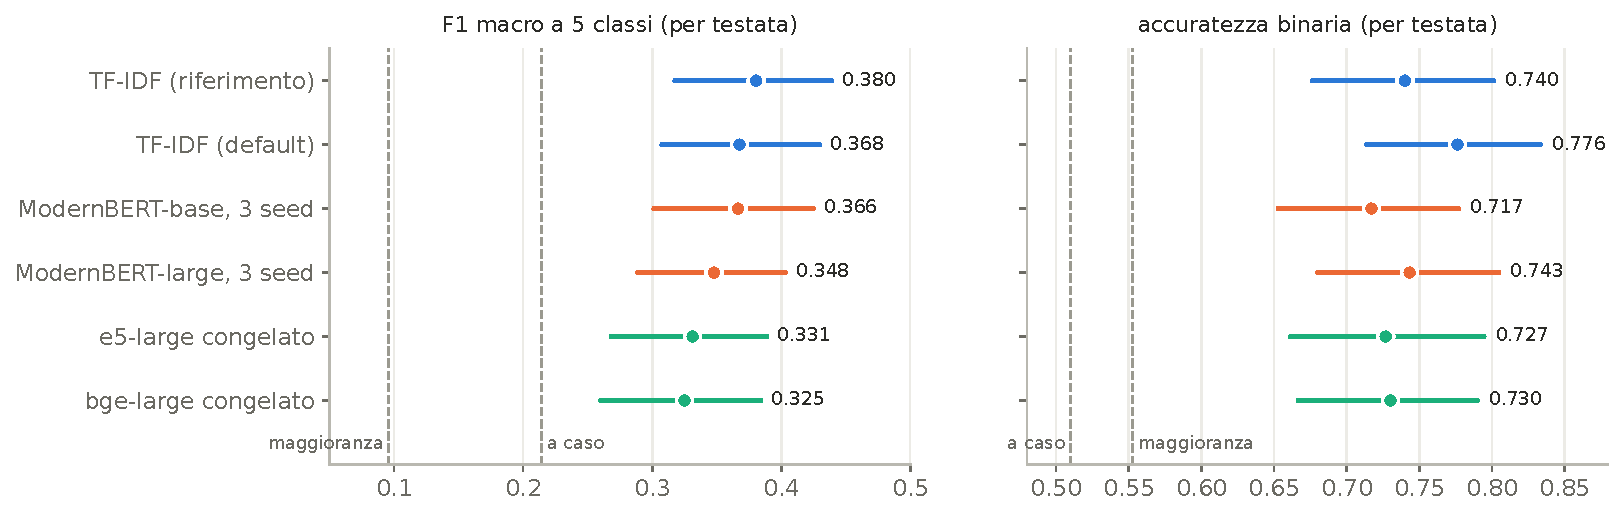
\includegraphics[width=\textwidth]{fig_risultati_intervalli.pdf}\\[0.2em]
  {\footnotesize Intervalli al 95\% con un bootstrap per gruppo: le differenze tra i modelli stanno tutte dentro.}
\end{frame}

\begin{frame}{Chi riconosce cosa}
  \begin{columns}[c]
    \begin{column}{0.6\textwidth}
      \centering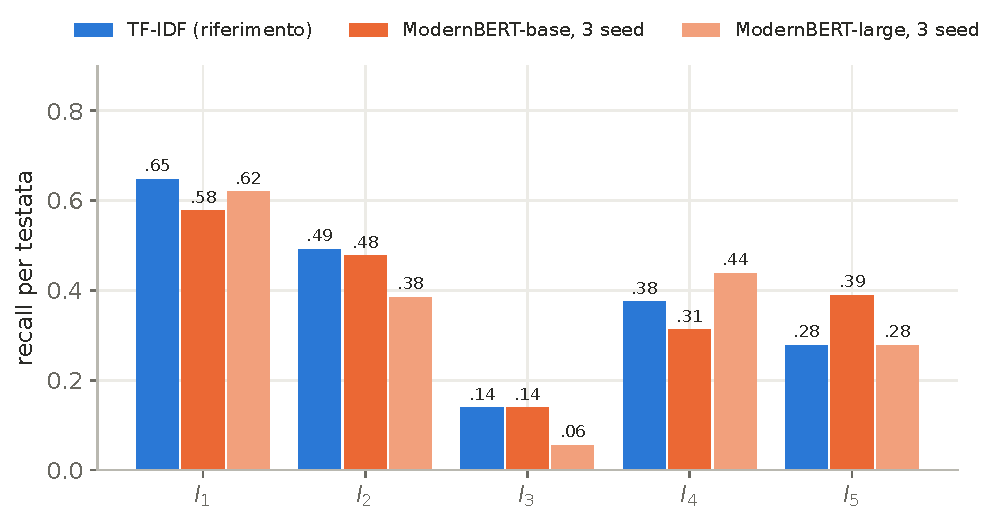
\includegraphics[width=\textwidth]{fig_recall_livelli.pdf}
    \end{column}
    \begin{column}{0.4\textwidth}
      \begin{itemize}[<+->]
        \setlength\itemsep{0.6em}
        \small
        \item Il TF-IDF riconosce meglio le testate \hl{inaffidabili} ($l_1$), ModernBERT le \hl{pi\`u affidabili} ($l_4$, $l_5$): sbagliano in modo \hl{diverso}
        \item Il vantaggio del TF-IDF su $l_1$ \hl{non viene dalle reti}: indovina le $l_1$ isolate (30/43) e quelle in un gruppo (20/28) allo stesso modo
        \item Il perch\'e lo spiega l'analisi pi\`u avanti: il TF-IDF legge il \hl{genere} della testata
      \end{itemize}
    \end{column}
  \end{columns}
\end{frame}

% ===================================================================================================
\divider{Come ho provato a battere il TF-IDF}{tre tentativi dopo la Versione 1, 19--22 ottobre}

\begin{frame}{Quattro versioni, lo stesso risultato}
  \centering\footnotesize
  \resizebox{\textwidth}{!}{%
  \begin{tabular}{llccc}
    \toprule
    & \textbf{L'idea} & \textbf{TF-IDF} & \textbf{ModernBERT} & \textbf{$\Delta$ [IC 95\%]} \\
    \midrule
    \textbf{V1} & la pipeline pulita (reti, gruppi, fold per gruppo) & 0,380 & 0,366 & $-0{,}01$ [$-0{,}07$; $+0{,}04$] \\
    \textbf{V2} & pi\`u pulizia e pi\`u testate nel training & 0,370 & 0,341 & $-0{,}03$ [$-0{,}10$; $+0{,}04$] \\
    \textbf{V3} & togliere il genere: affidabile s\`i/no dentro ogni orientamento$^{*}$ & 0,593 & 0,551 & $-0{,}04$ [$-0{,}10$; $+0{,}02$] \\
    \textbf{V4} & il titolo letto con l'articolo, i criteri NewsGuard come etichette & 0,390 & 0,360 & $-0{,}03$ [$-0{,}10$; $+0{,}04$] \\
    \bottomrule
  \end{tabular}}\\[0.4em]
  \raggedright{\scriptsize\itshape F1 macro per testata (V3: accuratezza bilanciata media sugli orientamenti$^{*}$), 304 testate, fold per gruppo; ModernBERT = ensemble di 3 seed (V3: 5); $\Delta$ con bootstrap per gruppo.}\\[0.6em]
  \centering\small Il TF-IDF resta sempre \hl{un po' avanti}, mai in modo significativo.
\end{frame}

% ---------------------------------------------------------------- V2
\begin{frame}{V2 --- pi\`u pulizia e pi\`u dati}
  \begin{itemize}
    \setlength\itemsep{0.6em}
    \item \hl{Cosa}: via i resti di link e tweet incorporati (il TF-IDF li usava per $l_1$); nel training anche le testate escluse dal tetto, \hl{863} invece di 304; una combinazione TF-IDF + ModernBERT
    \item \hl{Risultato}: TF-IDF 0,370, ModernBERT 0,341, combinazione 0,355. Niente cambia
    \item \hl{Perch\'e ha fallito}: i resti di link non erano il motivo del vantaggio del TF-IDF, e pi\`u testate della stessa rete non insegnano niente di nuovo
  \end{itemize}
\end{frame}

\begin{frame}{V2 --- l'analisi: che cosa legge il TF-IDF}
  \begin{columns}[c]
    \begin{column}{0.46\textwidth}
      \centering\footnotesize
      \begin{tabular}{lc}
        \toprule
        \textbf{Il TF-IDF su\dots} & \textbf{F1} \\
        \midrule
        il testo intero & 0,387 \\
        senza nomi propri & 0,383 \\
        \textbf{solo parole funzione} & \textbf{0,364} \\
        \midrule
        \textbf{solo metadati NewsGuard} & \textbf{0,339} \\
        \bottomrule
      \end{tabular}
    \end{column}
    \begin{column}{0.54\textwidth}
      \begin{itemize}
        \setlength\itemsep{0.5em}
        \footnotesize
        \item Il segnale \`e \hl{sparso}: regge senza nomi e con le sole parole funzione
        \item Segue il \hl{genere} della testata: $l_1$ = estrema destra e complotti, $l_2$ = destra di parte, $l_4$/$l_5$ = testate internazionali e d'inchiesta
        \item I soli metadati (orientamento, paese, tipo), senza testo, fanno quasi quanto lui
      \end{itemize}
    \end{column}
  \end{columns}
  \vspace{0.6em}
  \centering\small\itshape Un segnale lessicale e diffuso: il TF-IDF lo prende tutto, al transformer resta poco.
\end{frame}

% ---------------------------------------------------------------- V3
\begin{frame}{V3 --- togliere il genere}
  \begin{itemize}
    \setlength\itemsep{0.6em}
    \item \hl{Cosa}: compito binario (affidabile s\`i/no), pesi che rendono l'orientamento politico inutile per indovinare, valutazione \hl{dentro} ogni orientamento (i soli metadati fanno 0,50)
    \item \hl{Risultato}: TF-IDF 0,59--0,62, ModernBERT 0,55 (ensemble di 5 seed), embedding congelati 0,50--0,57
    \item \hl{Perch\'e ha fallito}: oltre il genere resta un segnale modesto ed \`e \hl{stile} (il TF-IDF sulle sole parole funzione fa 0,618, come sul testo intero): di nuovo lessicale
    \item[] {\small\itshape Unico indizio a favore: nell'orientamento Slightly Right tutti i seed di ModernBERT battono il TF-IDF (0,57--0,71 contro 0,51). Su 78 testate, a posteriori.}
  \end{itemize}
\end{frame}

% ---------------------------------------------------------------- V4
\begin{frame}{V4 --- quello che un TF-IDF non vede}
  \begin{itemize}
    \setlength\itemsep{0.6em}
    \item \hl{Cosa}: ModernBERT legge \hl{titolo [SEP] articolo}, cos\`i pu\`o confrontarli (``titoli ingannevoli'' \`e un criterio NewsGuard); in pi\`u impara i 5 criteri NewsGuard visibili nel testo come etichette in pi\`u
    \item \hl{Risultato}: ModernBERT da 0,341 a 0,356 con il titolo, 0,360 con i criteri. Ma il TF-IDF con il titolo passa da 0,370 a \hl{0,390}
    \item \hl{Perch\'e ha fallito}: il titolo aiuta tutti e due allo stesso modo, quindi il distacco resta; i criteri aggiungono pochissimo. Tra un seed e l'altro ModernBERT varia di 4 punti, pi\`u di ogni effetto trovato
  \end{itemize}
\end{frame}

% ===================================================================================================
\divider{Oltre il testo}{link citati e pagina HTML (tentativo 09, 22--23 ottobre)}

\begin{frame}{L'idea}
  \begin{itemize}
    \setlength\itemsep{0.55em}
    \small
    \item Non solo \hl{che cosa scrive} una testata, ma \hl{chi cita} e \hl{com'\`e fatto il suo sito}, tutto dall'HTML gi\`a scaricato. Una riga per testata, tre famiglie:
    \item[] \hl{testo}: la media TF-IDF dei suoi articoli (e, in pi\`u, ModernBERT: 3 semi)
    \item[] \hl{link}: i domini citati negli articoli e l'affidabilit\`a dei siti citati (dalle sole etichette del training)
    \item[] \hl{pagina}: tracker e pubblicit\`a, pagine di trasparenza (chi siamo, rettifiche, redazione\dots), firma, paywall, video incorporati
    \item \hl{Modelli} (regressioni logistiche): uno per famiglia; uno che le \hl{combina} (stacking sulle probabilit\`a fuori fold); uno \hl{``alla NewsGuard''} che stima i 9 criteri e somma i punti pubblici
    \item I criteri \hl{non} entrano mai come ingresso: il punteggio \`e esattamente la loro somma pesata, per tutte le 9.222 testate NewsGuard
    \item \hl{Stessa valutazione}: 301 testate, gruppi reti $\cup$ owner $\cup$ Parent Domain, bootstrap per gruppo. Riferimento: il TF-IDF per articolo, ricalcolato
  \end{itemize}
\end{frame}

\begin{frame}{I risultati}
  \centering\footnotesize
  \begin{tabular}{lccc}
    \toprule
    \textbf{Modello} & \textbf{F1 a 5 livelli} & \textbf{$\Delta$ dal riferimento [IC 95\%]} & \textbf{binario} \\
    \midrule
    \hl{riferimento}: TF-IDF per articolo & \hl{0,340} & --- & 0,684 \\
    testo (TF-IDF per testata) & 0,339 & $-0{,}00$ [$-0{,}05$; $+0{,}04$] & 0,684 \\
    ModernBERT (3 semi) & 0,325 & $-0{,}02$ [$-0{,}07$; $+0{,}04$] & 0,708 \\
    link & 0,247 & \wrong{$-0{,}09$ [$-0{,}15$; $-0{,}03$]} & 0,641 \\
    pagina & 0,241 & \wrong{$-0{,}10$ [$-0{,}16$; $-0{,}03$]} & 0,615 \\
    \midrule
    combinato testo + pagina & \hl{0,354} & $+0{,}01$ [$-0{,}06$; $+0{,}09$] & 0,711 \\
    combinato tutte & 0,347 & $+0{,}01$ [$-0{,}07$; $+0{,}09$] & 0,688 \\
    combinato tutte + ModernBERT & 0,318 & $-0{,}02$ [$-0{,}10$; $+0{,}05$] & 0,714 \\
    alla NewsGuard & 0,319 & $-0{,}02$ [$-0{,}10$; $+0{,}06$] & \hl{0,718} \\
    \bottomrule
  \end{tabular}\\[0.5em]
  \raggedright\scriptsize\itshape Per testata, 301 testate valutate. Maggioranza: F1 0,096, binario 0,561; a caso: F1 0,176. In rosso: significativamente peggio del riferimento.\\[0.6em]
  \centering\small\upshape Nessun modello batte il testo in modo significativo; link e pagina da soli hanno segnale, ma meno del testo.
\end{frame}

\begin{frame}{Che cosa si riesce a stimare}
  \begin{columns}[T]
    \begin{column}{0.45\textwidth}
      \centering\footnotesize
      \begin{tabular}{lc}
        \toprule
        \textbf{Criterio (alla NewsGuard)} & \textbf{acc.\ bil.} \\
        \midrule
        informazione responsabile & 0,77 \\
        titoli non ingannevoli & 0,72 \\
        corregge gli errori & 0,70 \\
        niente contenuti falsi & 0,67 \\
        firma gli articoli & 0,63 \\
        dice chi comanda & 0,62 \\
        notizie e opinioni & 0,61 \\
        propriet\`a e finanziamento & 0,56 \\
        segnala la pubblicit\`a & 0,54 \\
        \bottomrule
      \end{tabular}\\[0.4em]
      \raggedright\scriptsize Si stimano i criteri di \hl{contenuto}, non quelli \hl{di pagina}: proprio il contrario di quello che ci aspettavamo
    \end{column}
    \begin{column}{0.53\textwidth}
      \footnotesize
      \textbf{I segnali pi\`u forti}
      \begin{itemize}
        \setlength\itemsep{0.3em}
        \item \hl{l5} cita bbc.com, apple.news, siti governativi (army.mil, canada.ca, mod.uk); ha redazione, rettifiche, paywall, newsletter
        \item \hl{l1} cita t.me, gab.com, rt-english.com, pravda.ru; incorpora video da Rumble, Brighteon e simili
        \item \hl{l2} cita twitter.com, dailywire.com, rasmussenreports.com; ha pi\`u circuiti pubblicitari
        \item qualche segnale spurio (link riscritti dai filtri email: urldefense, proofpoint)
      \end{itemize}
    \end{column}
  \end{columns}
\end{frame}

\begin{frame}{Che cosa ne concludiamo}
  \begin{itemize}
    \setlength\itemsep{0.6em}
    \small
    \item Testo letto in due modi, link, pagina, criteri: \hl{tutto arriva allo stesso tetto}, F1 circa 0,34 e binario circa 0,70
    \item Link e pagina hanno segnale, ma \hl{non aggiungono} al testo: probabilmente raccontano di nuovo il genere della testata, che il testo vede gi\`a
    \item La \hl{variabilit\`a dei fold} \`e grande quanto le differenze tra modelli: con i gruppi nuovi (Parent Domain) il riferimento passa da 0,357 a 0,340 sulle stesse 284 testate, e 118 di loro cambiano previsione
    \item Con 301 testate in 218 gruppi non si distinguono differenze sotto i 6--7 punti
    \item Per il paper: con una valutazione che tiene conto delle reti, il tetto non dipende dal segnale; lo 0,68 che si ottiene senza gruppi era fuga tra training e test
    \item Possibile passo successivo: ripetere tutto con pi\`u divisioni in fold, per stringere gli intervalli (solo CPU, circa un'ora a divisione)
  \end{itemize}
\end{frame}

\end{document}
